\chapter{Overall description}
\section{Product perspective}
\subsection{Scenarios}

\begin{enumerate}
	\descitem{CPO wants to start using the platform}\\
	Antony, the owner of two charging stations, wants to optimize their use and join the e-Charging ecosystem. He contacts customer service and arranges for the installation of a CMPS on a cloud server. Antony then connects his stations to the internet, connecting each charging slot. With the assistance of technicians, he inputs all the necessary information into the system to ensure it can effectively manage his two charging stations. After the installation is completed, Antony accesses the CPMS portal and offers a discount on the prices he charges to celebrate the new system. The eMSP network is notified of the presence of the new CPMS. The DSOs located at the various stations are also connected, allowing for dynamic selection of the energy source\\\\
	
	\descitem{CPO wants to change the price of the energy sold}\\
	Alice is the administrator of a charging station and has decided to increase the price of energy. Alice opens the internet portal of her CPMS via a browser. By entering the credentials, Alice accesses the interface concerning the proposed price. After a careful analysis, Alice changes the price and presses the "Save Changes" button.\\\\
	
	\descitem{CPO wants to disable a charging socket to perform maintenance}\\
	Fabio is a CPO and has to carry out routine checks on the correct functioning of a charging socket. Fabio opens the internet portal of her CPMS via a browser. By entering the credentials, Fabio accesses the booking interface. Fabio selects an available time slot and presses the "Maintenance" button.\\
	
	\descitem{eMSP wants to start a charge at the CP}
	eMSP wants to start a new charging session, but without having a reservation at the indicated charging point. Then it sent an immediate booking request for a charging slot to the system. The system verifies that there is availability in that particular station. Since there is availability, the system adds the session to the schedule and sends a confirmation message to the eMSP.\\
	
	
	\descitem{eMSP wants to be notified at the end of the charge}\\
	The eMSP wants to receive information regarding the status of the current charging session identified by a booking\_id. The system therefore every time it receives information on the status of the session from the charging slot, notifies the eMSP about the status.\\
	
\end{enumerate}

\newpage

\subsection{Class Diagram}

\begin{figure}[h]
\centering
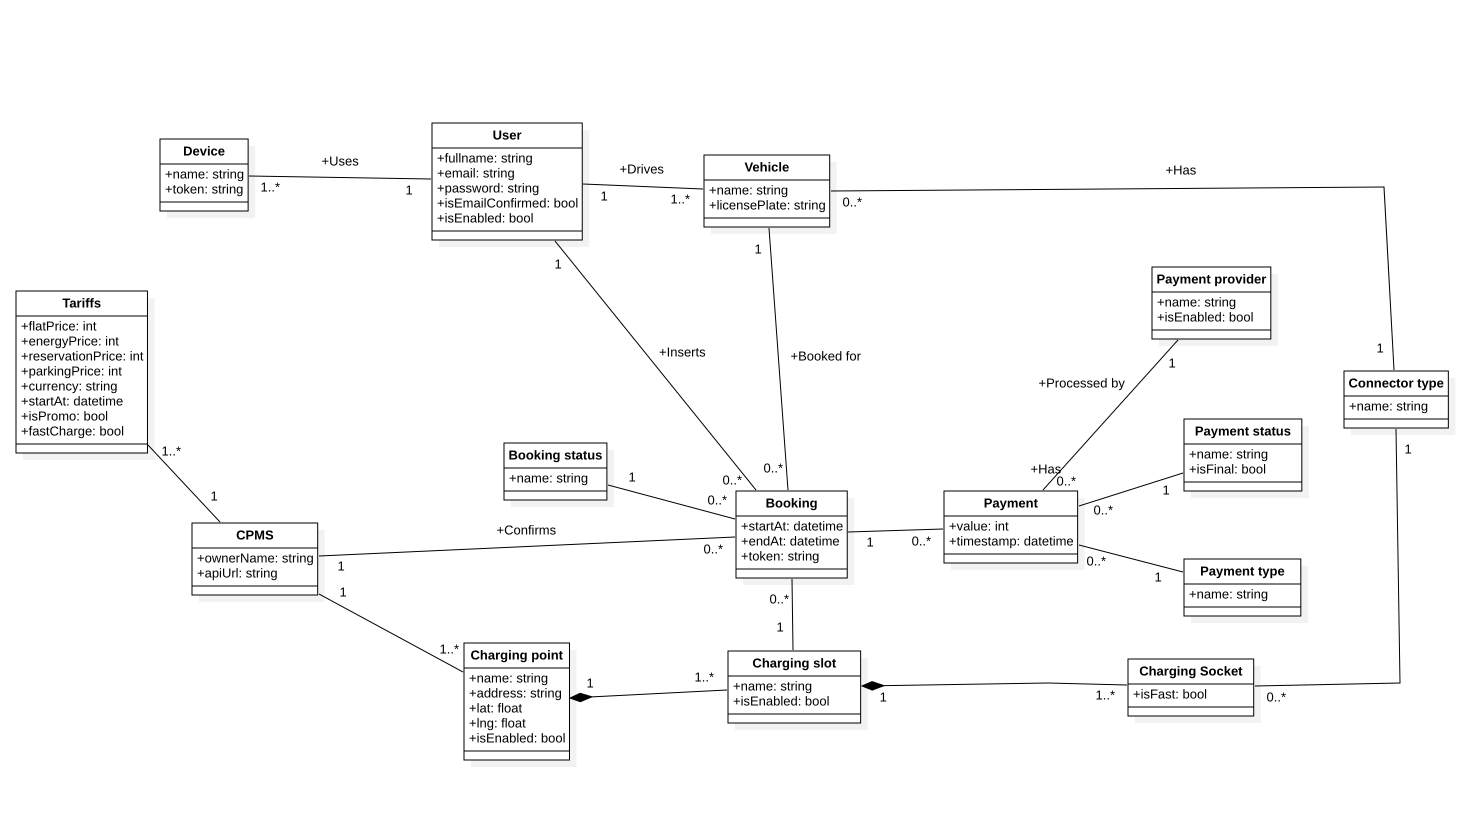
\includegraphics[width=\textwidth]{class_diagram}
\caption{Class diagram of the CPMS system for eMall}
\end{figure}

\clearpage
\newpage

\subsection{State charts}

\begin{figure}[h]
\centering
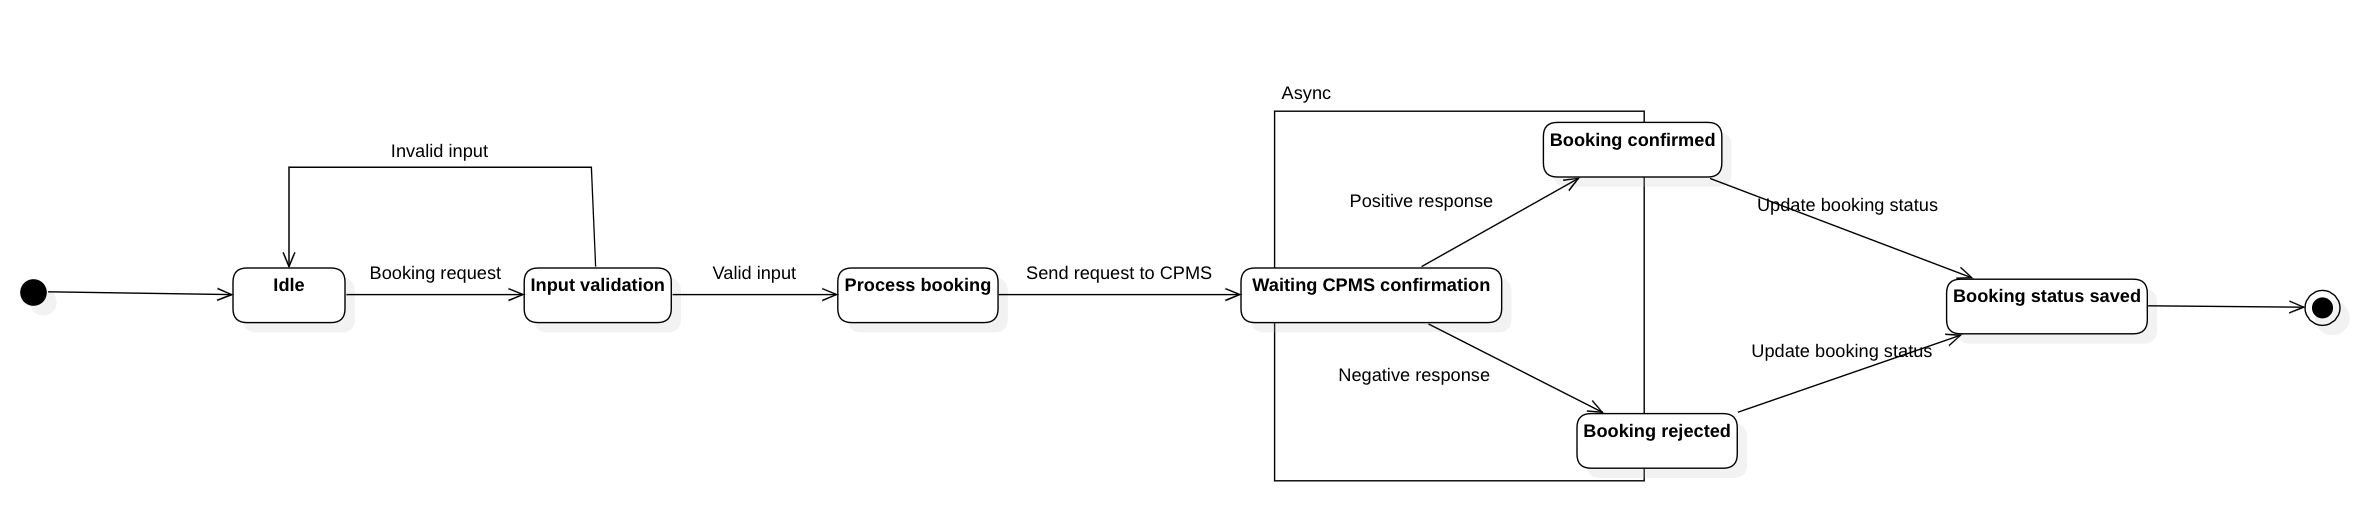
\includegraphics[width=\textwidth]{booking_state_diagram}
\caption{State diagram for Booking}
\end{figure}

\begin{figure}[h]
\centering
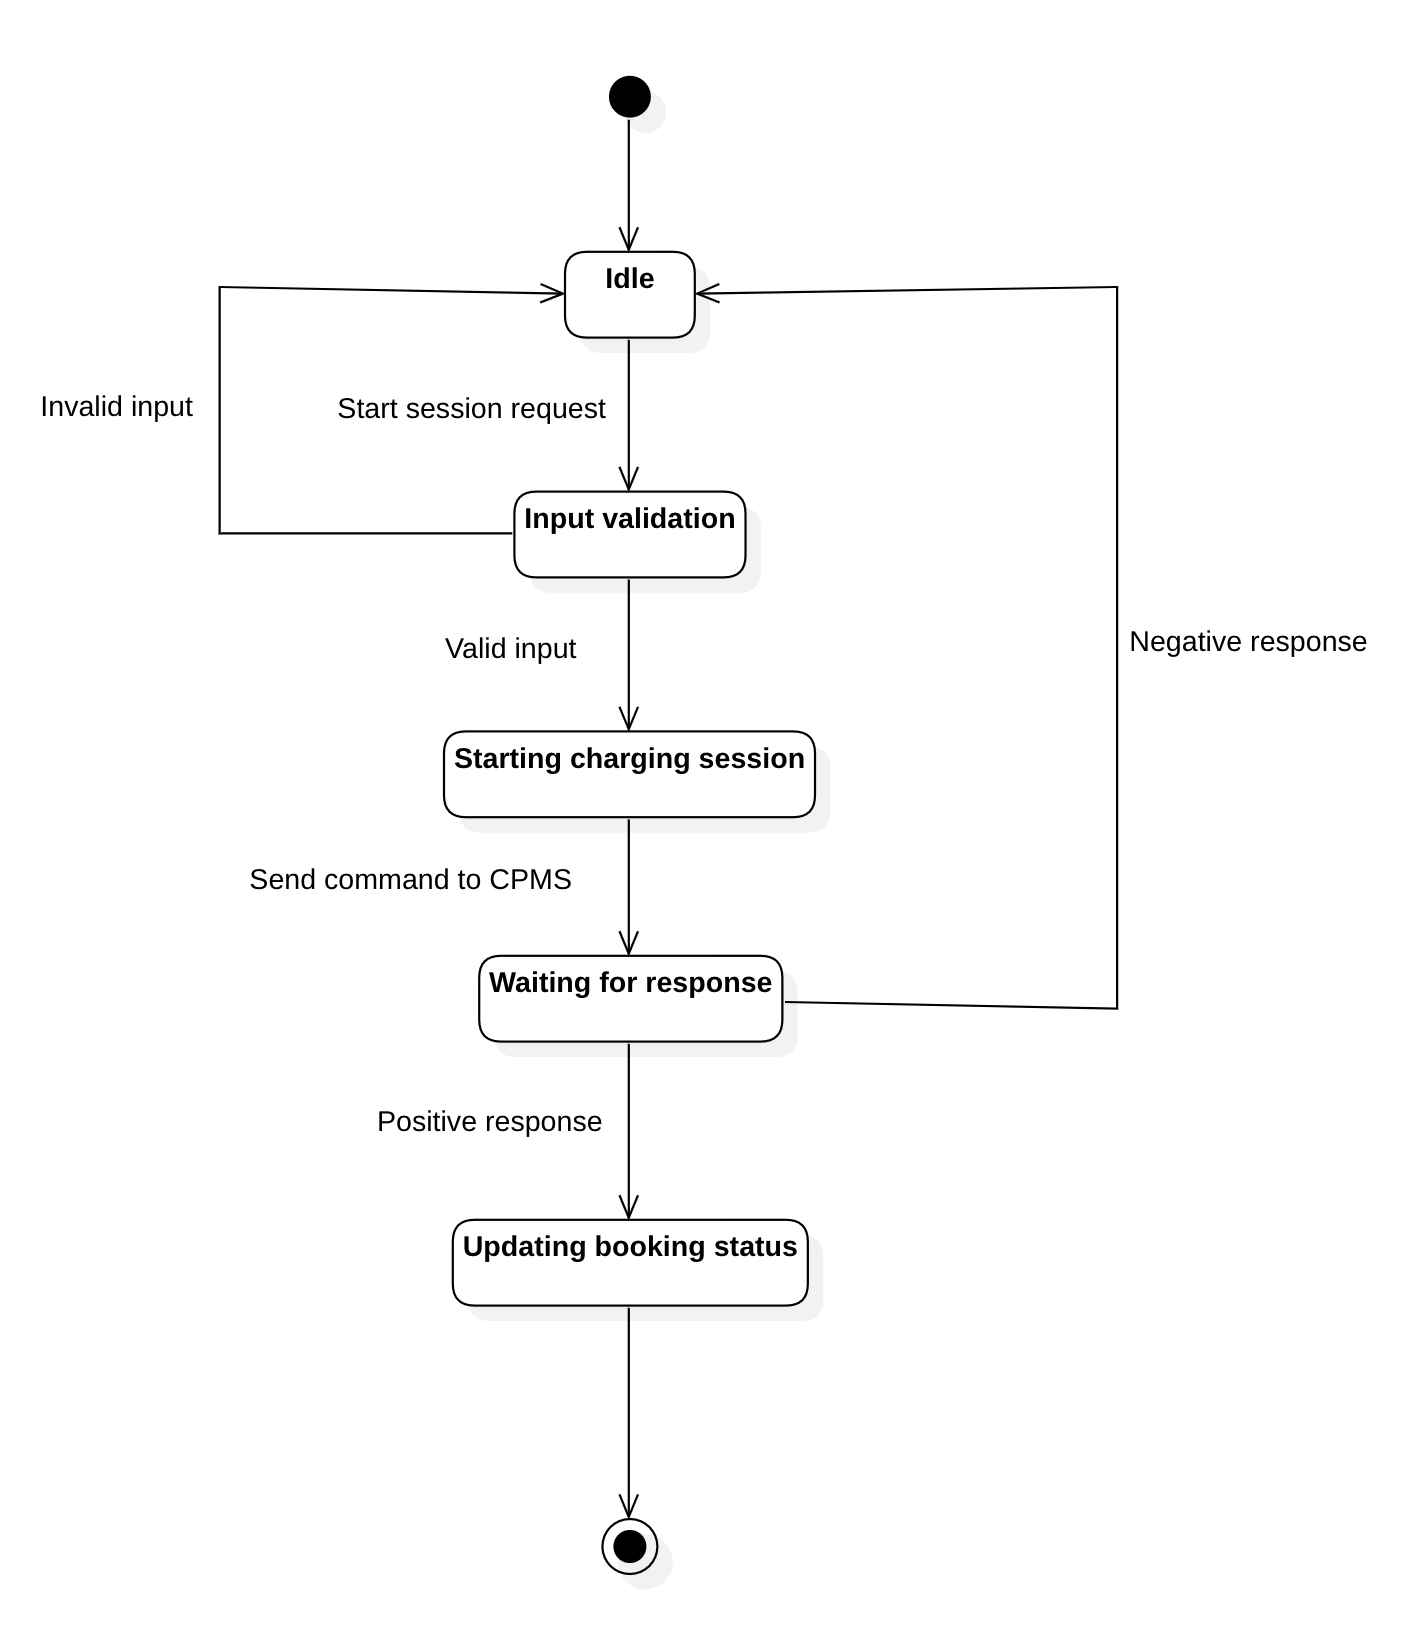
\includegraphics[width=\textwidth]{charging_session_state_diagram}
\caption{State diagram for a Charging Session}
\end{figure}

\begin{figure}[h]
\centering
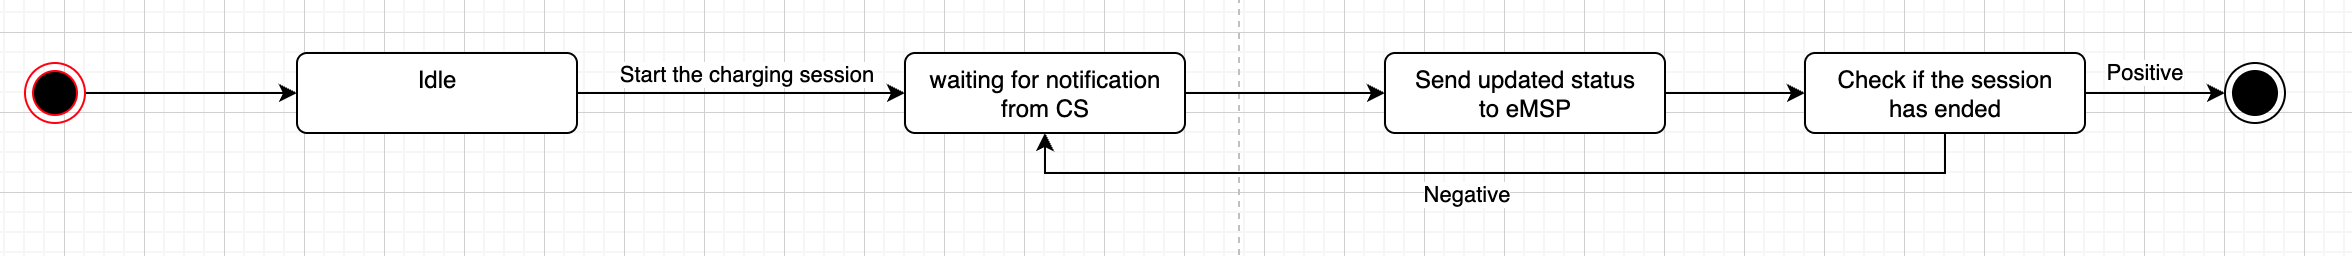
\includegraphics[width=\textwidth]{charging_session_status}
\caption{State diagram for monitor session status}
\end{figure}

\clearpage
\newpage


\section{Product functions}
In this section the main functionalities of the CPMS is presented and described in more detail.\\

\begin{itemize}
	\item As OCPI enables a very complex pricing system, to keep the scope of the project simple, the system will use only the per-KW price (also called energy based price), with differentiation between fast charging and non-fast charging. Time limited promotions are also allowed.The prices are synced by the CPMSs via the PUSH interface defined in the OCPI protocol. (i.e. at any time, each CPMS can define only two active prices: standard and fast-charging). 
	\item Another limitation that we need to impose to reduce the complexity is the various connector types. We define only two generic types of connector: standard and fast-charging, each type has its own pricing defined by the CPMS.
\end{itemize}

\subsection{Dynamically decide the energy source to use}
The dynamic management of the needed energy resources is one of the CPMS's main responsibilities. It should also be able to dynamically decide from which DSO to acquire energy based on the current price and energy source mix, and decide whether to store or use energy from the station's batteries. 

\subsection{Communicate information to the various eMSPs}
The system must be able to communicate via the OCPI protocol with the various eMSPs that make port on the network. Through this protocol, the two actors will be able to communicate information such as: position of the charging stations managed by the CPO, rates offered, availability for reservations, type of charging available. \\

\subsection{CPOs, station monitoring and management}
It must be possible to monitor and display information such as: tariffs offered, current cost of energy purchased from DSOs, battery status, reservation schedules. Furthermore, the admin must be able, through a dedicated portal, to make changes and decisions on the management of the station.

\subsection{Manage the reservations schedule}
The system should be able to manage and keep track of the reservations that are made by the various eMSPs. The system must be able to handle the modification, if possible, or cancellation of reservations.

\subsection{Interaction with DSOs}
The system must be able to communicate with the various Distribution Management Systems (DSOs). The system must be able to request information such as: energy price, energy type. It must also be able to request connection and supply of energy from each DSO.

\subsection{Communication with the charging slots}
The system should be able to communicate with the charging slots present in each charging point. communication must take place via the OCPP protocol. The exchange of information such as: diagnostic data, charging status, activation of the charging socket must take place through this protocol.

\section{User characteristics}
We can identify a CPO administrator as the only user of the CPMS system. For the purpose of the project we assume that situations in which the CPO administrator is not present or registered are not allowed.

\begin{enumerate}
	\descitem{CPO Administrators}
	The CPO will utilize the CPMS to oversee their charging stations and manually address tasks such as selecting which DSO to obtain energy from or establishing special offers for charging stations. 
	
	\descitem{Maintainer}
	A person responsible for maintaining and repairing all parts of the charging station.
	
\end{enumerate}

\section{Assumptions, dependencies and constraints}

\subsection{Assumptions}
\begin{tabular}{|l|l|}
	\hline
	D1 & There is a system admin that does the initial setup of the system and manages it \\
	\hline
	D2 & The system admin adds the necessary information about charging point, slots to the database \\
	\hline
	D3 & DSOs are connected and entered into the system by the admin during the initial set up\\
	\hline
	D4 & Users always complete their booked charging session\\
	\hline
\end{tabular}
